%Copyright (C) 2020  László Ady (NextTechnologies Complex System Research Institute)
%
%This document is free document: you can redistribute it and/or modify
%it under the terms of the GNU General Public License as published by
%the Free Software Foundation, either version 3 of the License, or
%(at your option) any later version.
%
%This program is distributed in the hope that it will be useful,
%but WITHOUT ANY WARRANTY; without even the implied warranty of
%MERCHANTABILITY or FITNESS FOR A PARTICULAR PURPOSE.  See the
%GNU General Public License for more details.
%
%You should have received a copy of the GNU General Public License
%along with this program.  If not, see <https://www.gnu.org/licenses/>.
%
%Contributors:
%  László Ady <adylaszlo@nexttechnologies.hu>  base editing
%
%------------------------------------------------------------------------------------------

\documentclass{standalone}
\usepackage{tikz}
\usepackage[utf8]{inputenc}
\usetikzlibrary{intersections}


\def \complexSystemStr {Komplex rendszer}
\def \emergenceStr {Emergencia}
\def \selfOrganisationStr {Önszerveződés}

\def \overScaleStr {térben}
\def \overTimeStr {időben}

\def \collectiveBehavionStr {Kollektív\\viselkedés}
\def \networksStr {Hálózat}
\def \evolutionAdaptionStr {Evolució \&\\adaptáció}
\def \patetrnFormationStr {Mintázat\\kialakulás}
\def \systemTheoryStr {Rendszer\\elmélet}
\def \nonLinearDynamicsStr {Nem lineális\\dinamika}
\def \gameTheoryStr {Játék\\elmélet}

\def \socialDynamicsStr {Társas dinamika}
\def \collectiveIntelligenceStr {Kollektív intelligencia}
\def \selfOrganisedCriticalityStr {Önszervezett kritika}
\def \herdMentalityStr {Csorda\\szellem}
\def \phaseTransitionStr {Fázis\\átmenet}
\def \syncronizationStr {Szinkronizáció}
\def \antColonyOptimalisationStr {Hangya kolónia optimalizáció}
\def \particleSwarnOptimalisationStr {Részecske raj optimalizáció}
\def \swarnBehavionStr {Raj viselkedés}
\def \agentBasedModellingStr {Ügynök\\alapú\\modellezés}


\def \bigCircleDiameter {14}
\def \smallCircleDiameter {4.22}


\begin{document}
\pagestyle{empty}
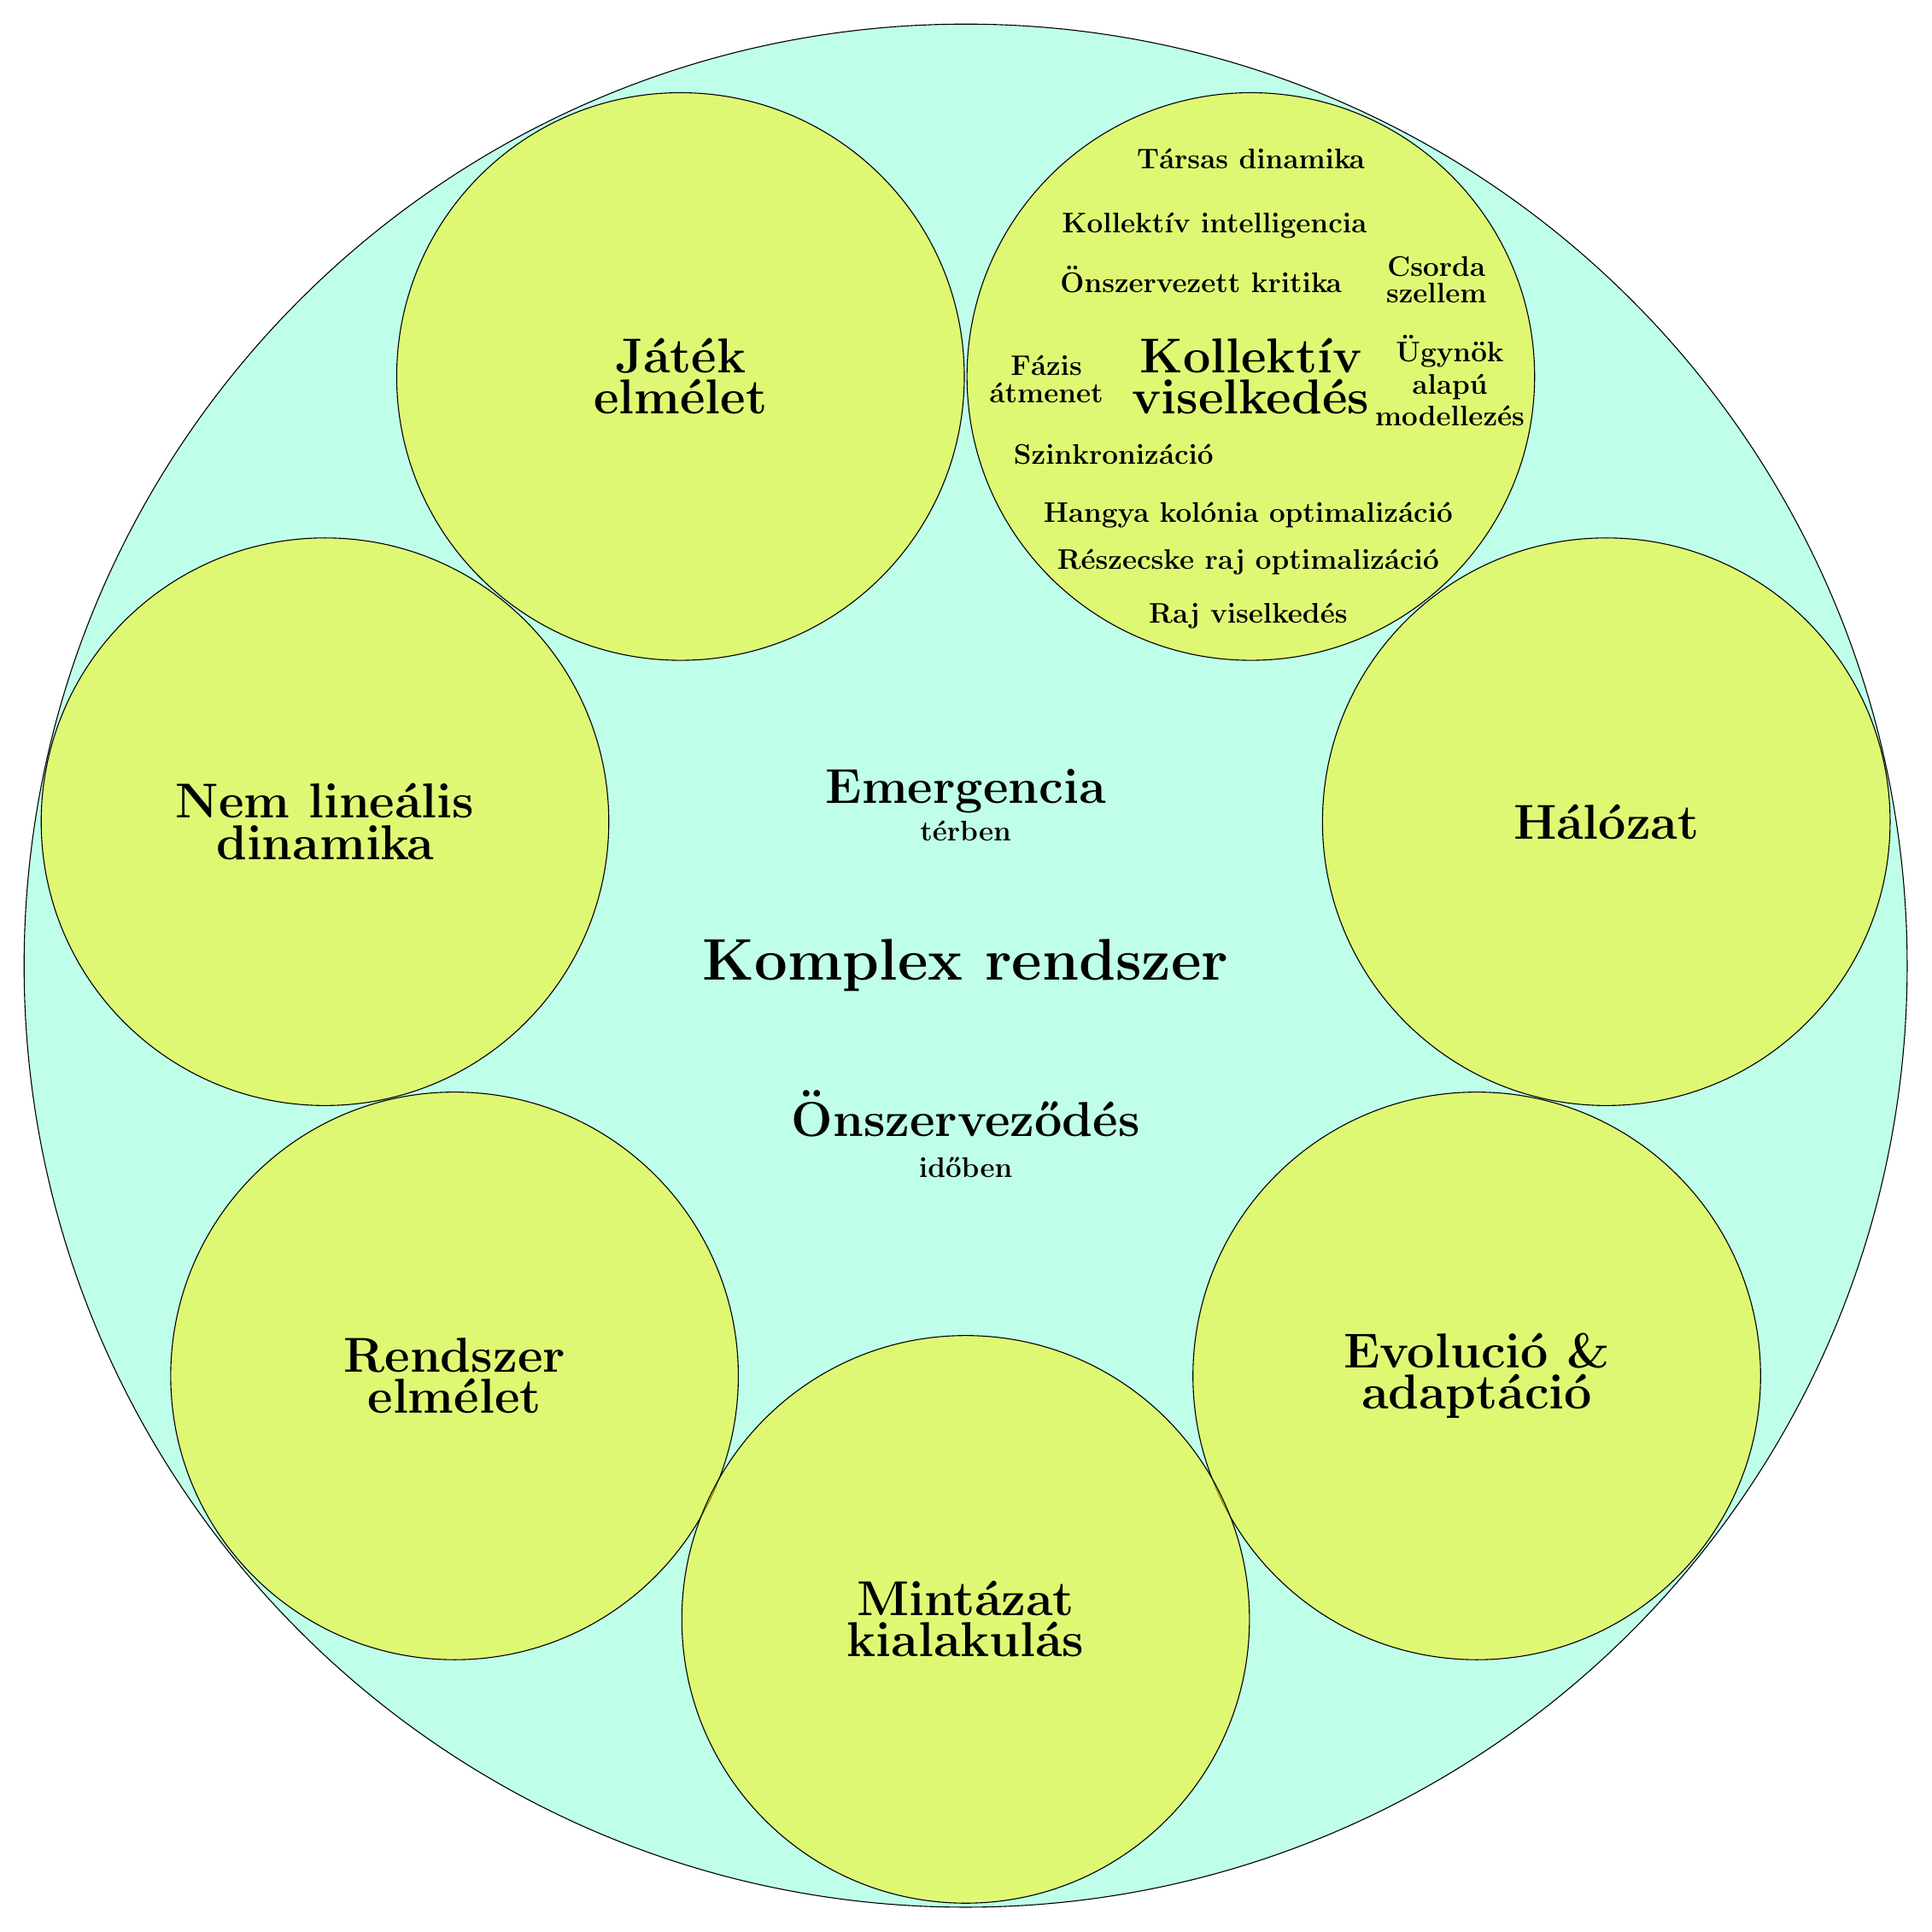
\begin{tikzpicture}


\definecolor{aquamarine}{rgb}{0.5, 1.0, 0.83}


\begin{scope}[shift={(3cm,-5cm)}, fill opacity=0.5,
  mytext/.style={text opacity=1,font=\large\bfseries}]



\draw[fill=aquamarine, draw = black] (0,0) circle ({\bigCircleDiameter});

\draw[fill=yellow, draw = black,name path=circle 1] (-4.24,8.76) circle ({\smallCircleDiameter});
\draw[fill=yellow, draw = black,name path=circle 2] (4.24,8.76) circle ({\smallCircleDiameter});

\draw[fill=yellow, draw = black,name path=circle 2] (-9.526,2.14) circle ({\smallCircleDiameter});
\draw[fill=yellow, draw = black,name path=circle 1] (9.526,2.14) circle ({\smallCircleDiameter});

\draw[fill=yellow, draw = black,name path=circle 1] (7.6,-6.1) circle ({\smallCircleDiameter});
\draw[fill=yellow, draw = black,name path=circle 2] (-7.6,-6.1) circle ({\smallCircleDiameter});

\draw[fill=yellow, draw = black,name path=circle 2] (0,-9.72) circle ({\smallCircleDiameter});


\node[mytext] at (0,0) {\Huge \complexSystemStr};
\node[mytext] at (0,2.6) {\huge \emergenceStr};
\node[mytext] at (0,2) {\overScaleStr};
\node[mytext] at (0,-2.2) {\huge \selfOrganisationStr};
\node[mytext] at (0,-3) {\overTimeStr};


\node[mytext] at (4.24,8.76) {\huge \shortstack{\collectiveBehavionStr}};
\node[mytext] at (-4.24,8.76) {\huge \shortstack{\gameTheoryStr}};

\node[mytext] at (-9.526,2.14) {\huge \shortstack{\nonLinearDynamicsStr}};
\node[mytext] at (9.526,2.14) {\huge \shortstack{\networksStr}};

\node[mytext] at (-7.6,-6.1) {\huge \shortstack{\systemTheoryStr}};
\node[mytext] at (7.6,-6.1) {\huge \shortstack{\evolutionAdaptionStr}};
\node[mytext] at (0,-9.72) {\huge \shortstack{\patetrnFormationStr}};

\node[mytext] at (4.24,12) {\shortstack{\socialDynamicsStr}};
\node[mytext] at (3.7,11) {\shortstack{\collectiveIntelligenceStr}};
\node[mytext] at (7,10.2) {\shortstack{\herdMentalityStr}};
\node[mytext] at (3.5,10.2) {\shortstack{\selfOrganisedCriticalityStr}};
\node[mytext] at (1.2,8.72) {\shortstack{\phaseTransitionStr}};
\node[mytext] at (2.2,7.6) {\shortstack{\syncronizationStr}};
\node[mytext] at (4.2,6.7) {\shortstack{\antColonyOptimalisationStr}};
\node[mytext] at (7.2,8.7) {\shortstack{\agentBasedModellingStr}};
\node[mytext] at (4.2,6.0) {\shortstack{\particleSwarnOptimalisationStr}};
\node[mytext] at (4.2,5.2) {\shortstack{\swarnBehavionStr}};


\end{scope}
\end{tikzpicture}

\end{document}
